\documentclass{standalone}
\usepackage{tikz}
\usetikzlibrary{patterns, positioning}
\usepackage[sfdefault]{ClearSans} %% option 'sfdefault' activates Clear Sans as the default text font
\usepackage[T1]{fontenc}

\begin{document}
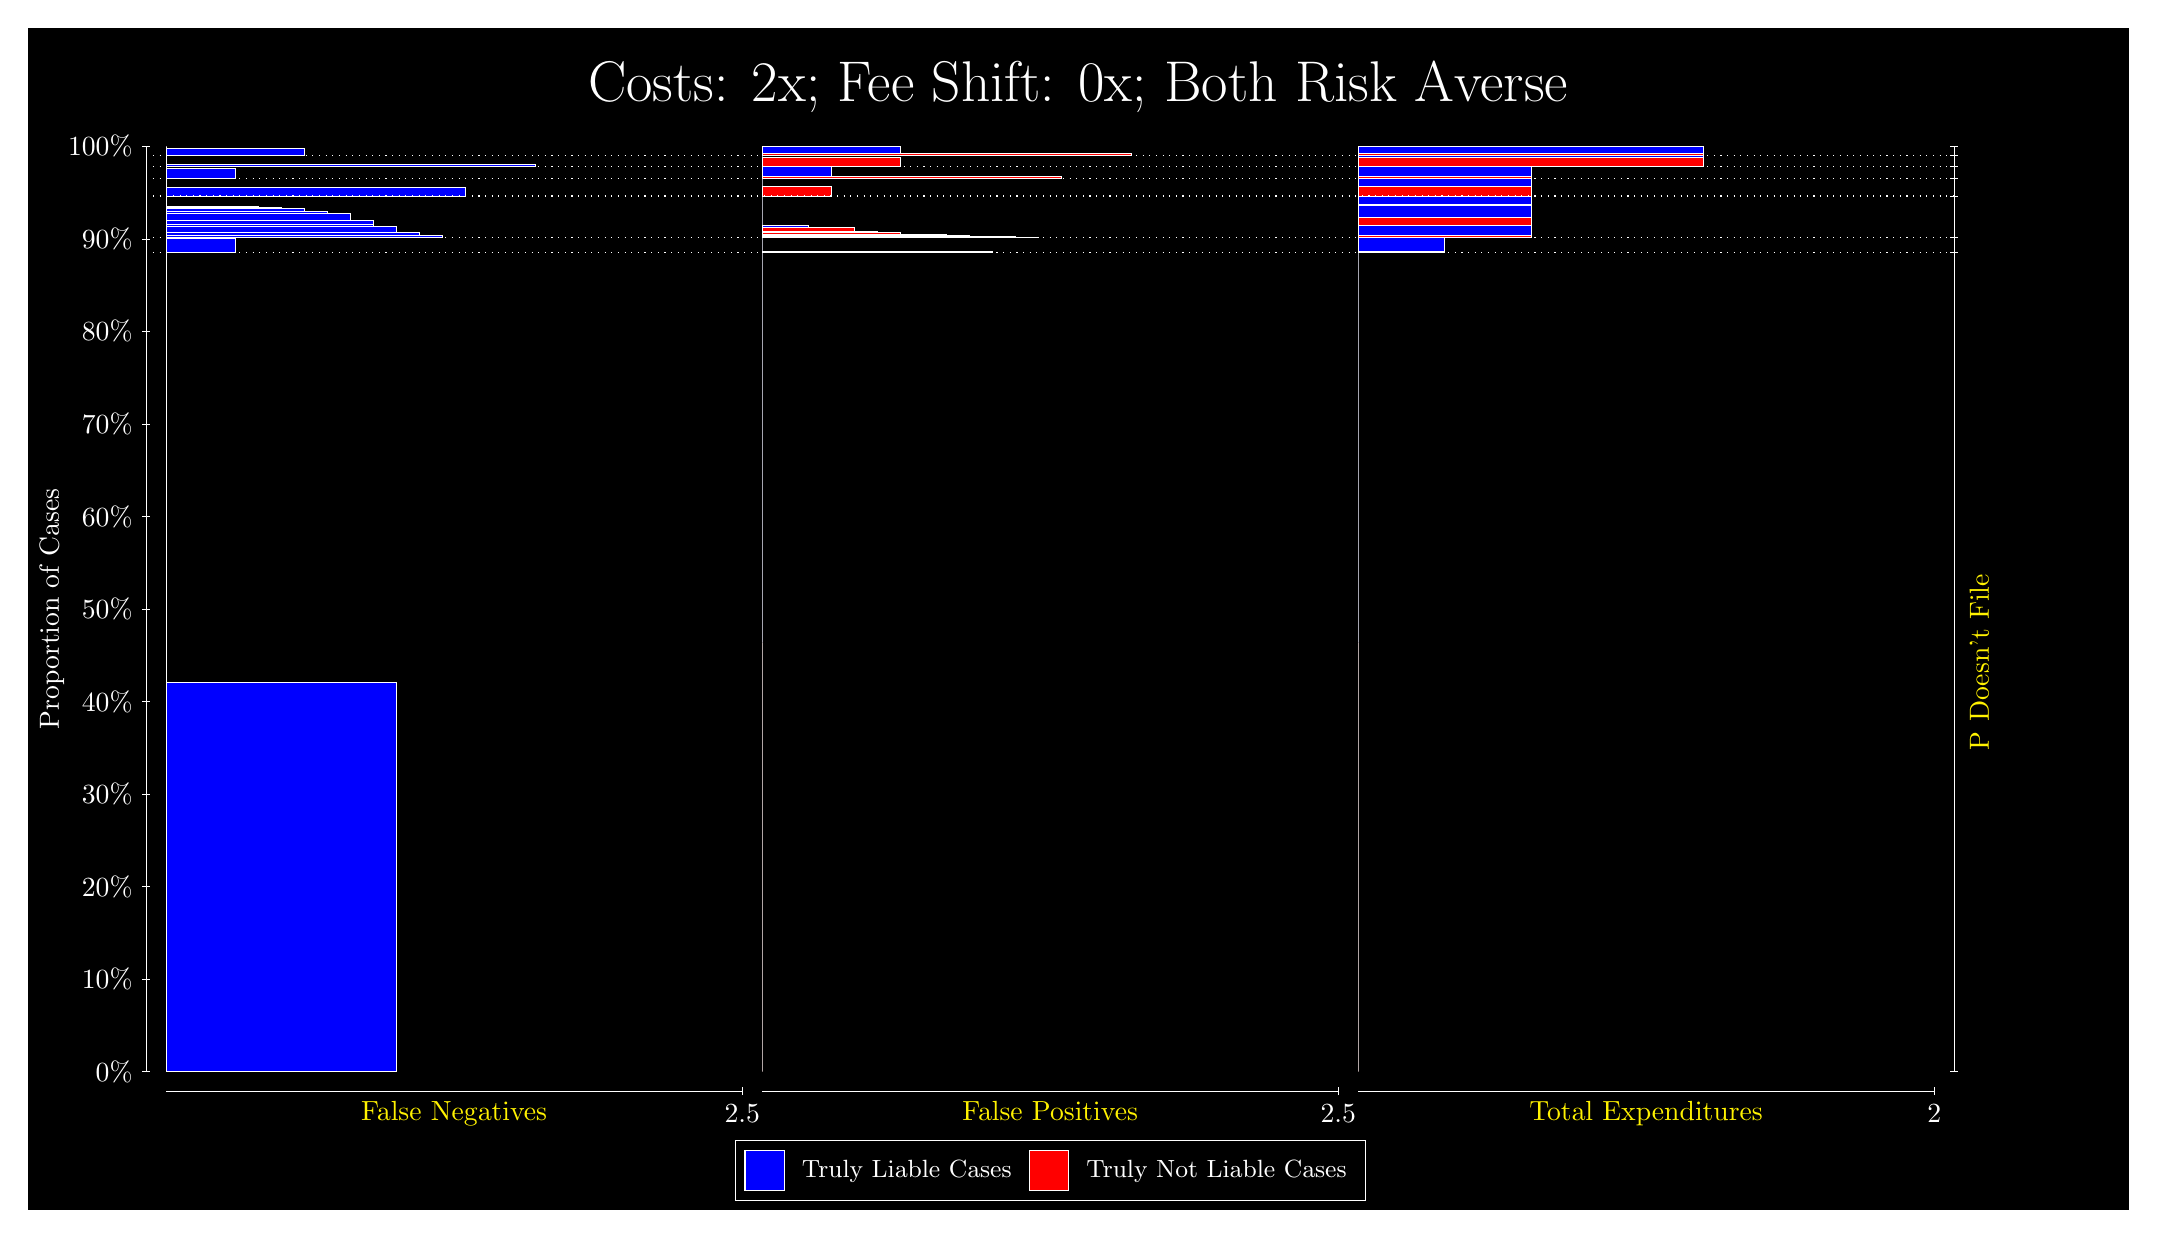
\begin{tikzpicture}
\draw[fill=black] (0,0) rectangle (26.667,15);
\draw[text=white] (0,13.5) rectangle (26.667,15) node[midway] {\huge Costs: 2x; Fee Shift: 0x; Both Risk Averse};
\draw[white, very thin] (1.5,1.75) -- (1.5,13.5);
\node[rotate=90, text=white, anchor=center] at (0.3, 7.625) {Proportion of Cases};
\draw[white, very thin] (1.45,1.75) -- (1.55,1.75);
\node[text=white, anchor=east] at (1.45, 1.75) {0\%};
\draw[white, very thin] (1.45,2.925) -- (1.55,2.925);
\node[text=white, anchor=east] at (1.45, 2.925) {10\%};
\draw[white, very thin] (1.45,4.1) -- (1.55,4.1);
\node[text=white, anchor=east] at (1.45, 4.1) {20\%};
\draw[white, very thin] (1.45,5.275) -- (1.55,5.275);
\node[text=white, anchor=east] at (1.45, 5.275) {30\%};
\draw[white, very thin] (1.45,6.45) -- (1.55,6.45);
\node[text=white, anchor=east] at (1.45, 6.45) {40\%};
\draw[white, very thin] (1.45,7.625) -- (1.55,7.625);
\node[text=white, anchor=east] at (1.45, 7.625) {50\%};
\draw[white, very thin] (1.45,8.8) -- (1.55,8.8);
\node[text=white, anchor=east] at (1.45, 8.8) {60\%};
\draw[white, very thin] (1.45,9.975) -- (1.55,9.975);
\node[text=white, anchor=east] at (1.45, 9.975) {70\%};
\draw[white, very thin] (1.45,11.15) -- (1.55,11.15);
\node[text=white, anchor=east] at (1.45, 11.15) {80\%};
\draw[white, very thin] (1.45,12.325) -- (1.55,12.325);
\node[text=white, anchor=east] at (1.45, 12.325) {90\%};
\draw[white, very thin] (1.45,13.5) -- (1.55,13.5);
\node[text=white, anchor=east] at (1.45, 13.5) {100\%};

\draw[white, very thin] (24.457,1.75) -- (24.457,13.5);
\draw[white, very thin] (24.407,1.75) -- (24.507,1.75);
\node[anchor=west] at (24.407, 1.75) {};
\draw[white, very thin] (24.407,12.149) -- (24.507,12.149);
\node[anchor=west] at (24.407, 12.149) {};
\draw[white, very thin] (24.407,12.347) -- (24.507,12.347);
\node[anchor=west] at (24.407, 12.347) {};
\draw[white, very thin] (24.407,12.869) -- (24.507,12.869);
\node[anchor=west] at (24.407, 12.869) {};
\draw[white, very thin] (24.407,13.096) -- (24.507,13.096);
\node[anchor=west] at (24.407, 13.096) {};
\draw[white, very thin] (24.407,13.247) -- (24.507,13.247);
\node[anchor=west] at (24.407, 13.247) {};
\draw[white, very thin] (24.407,13.385) -- (24.507,13.385);
\node[anchor=west] at (24.407, 13.385) {};
\draw[white, very thin] (24.407,13.5) -- (24.507,13.5);
\node[anchor=west] at (24.407, 13.5) {};

\draw[white, very thin, fill=blue] (1.75,1.75) rectangle (4.6775,6.6983);
\draw[white, very thin, fill=red] (1.75,6.6983) rectangle (1.75,12.149);
\draw[white, very thin, fill=blue] (1.75,12.149) rectangle (2.6283,12.329);
\draw[white, very thin, fill=red] (1.75,12.329) rectangle (1.75,12.347);
\draw[white, very thin, fill=blue] (1.75,12.347) rectangle (5.2631,12.376);
\draw[white, very thin, fill=blue] (1.75,12.376) rectangle (4.9703,12.406);
\draw[white, very thin, fill=blue] (1.75,12.406) rectangle (4.6775,12.485);
\draw[white, very thin, fill=blue] (1.75,12.485) rectangle (4.3848,12.507);
\draw[white, very thin, fill=blue] (1.75,12.507) rectangle (4.3848,12.557);
\draw[white, very thin, fill=blue] (1.75,12.557) rectangle (4.092,12.644);
\draw[white, very thin, fill=blue] (1.75,12.644) rectangle (3.7993,12.68);
\draw[white, very thin, fill=blue] (1.75,12.68) rectangle (3.5065,12.713);
\draw[white, very thin, fill=blue] (1.75,12.713) rectangle (3.2138,12.723);
\draw[white, very thin, fill=blue] (1.75,12.723) rectangle (2.921,12.738);
\draw[white, very thin, fill=red] (1.75,12.738) rectangle (1.75,12.869);
\draw[white, very thin, fill=blue] (1.75,12.869) rectangle (5.5558,12.978);
\draw[white, very thin, fill=red] (1.75,12.978) rectangle (1.75,13.096);
\draw[white, very thin, fill=blue] (1.75,13.096) rectangle (2.6283,13.226);
\draw[white, very thin, fill=red] (1.75,13.226) rectangle (1.75,13.247);
\draw[white, very thin, fill=blue] (1.75,13.247) rectangle (6.4341,13.275);
\draw[white, very thin, fill=red] (1.75,13.275) rectangle (1.75,13.385);
\draw[white, very thin, fill=blue] (1.75,13.385) rectangle (3.5065,13.475);
\draw[white, very thin, fill=red] (1.75,13.475) rectangle (1.75,13.5);
\draw[white, very thin, fill=red] (9.3189,1.75) rectangle (9.3189,7.2011);
\draw[white, very thin, fill=blue] (9.3189,7.2011) rectangle (9.3189,12.149);
\draw[white, very thin, fill=red] (9.3189,12.149) rectangle (12.246,12.168);
\draw[white, very thin, fill=blue] (9.3189,12.168) rectangle (9.3189,12.347);
\draw[white, very thin, fill=red] (9.3189,12.347) rectangle (12.832,12.35);
\draw[white, very thin, fill=red] (9.3189,12.35) rectangle (12.539,12.352);
\draw[white, very thin, fill=red] (9.3189,12.352) rectangle (12.246,12.358);
\draw[white, very thin, fill=red] (9.3189,12.358) rectangle (11.954,12.364);
\draw[white, very thin, fill=red] (9.3189,12.364) rectangle (11.661,12.377);
\draw[white, very thin, fill=red] (9.3189,12.377) rectangle (11.368,12.388);
\draw[white, very thin, fill=red] (9.3189,12.388) rectangle (11.075,12.41);
\draw[white, very thin, fill=red] (9.3189,12.41) rectangle (10.783,12.424);
\draw[white, very thin, fill=red] (9.3189,12.424) rectangle (10.49,12.478);
\draw[white, very thin, fill=blue] (9.3189,12.478) rectangle (9.9044,12.493);
\draw[white, very thin, fill=blue] (9.3189,12.493) rectangle (9.6116,12.503);
\draw[white, very thin, fill=blue] (9.3189,12.503) rectangle (9.3189,12.869);
\draw[white, very thin, fill=red] (9.3189,12.869) rectangle (10.197,12.988);
\draw[white, very thin, fill=blue] (9.3189,12.988) rectangle (9.3189,13.096);
\draw[white, very thin, fill=red] (9.3189,13.096) rectangle (13.125,13.117);
\draw[white, very thin, fill=blue] (9.3189,13.117) rectangle (10.197,13.247);
\draw[white, very thin, fill=red] (9.3189,13.247) rectangle (11.075,13.357);
\draw[white, very thin, fill=blue] (9.3189,13.357) rectangle (9.3189,13.385);
\draw[white, very thin, fill=red] (9.3189,13.385) rectangle (14.003,13.41);
\draw[white, very thin, fill=blue] (9.3189,13.41) rectangle (11.075,13.5);
\draw[white, very thin, fill=red] (16.888,1.75) rectangle (16.888,7.2011);
\draw[white, very thin, fill=blue] (16.888,7.2011) rectangle (16.888,12.149);
\draw[white, very thin, fill=red] (16.888,12.149) rectangle (17.986,12.168);
\draw[white, very thin, fill=blue] (16.888,12.168) rectangle (17.986,12.347);
\draw[white, very thin, fill=red] (16.888,12.347) rectangle (19.083,12.368);
\draw[white, very thin, fill=blue] (16.888,12.368) rectangle (19.083,12.499);
\draw[white, very thin, fill=red] (16.888,12.499) rectangle (19.083,12.593);
\draw[white, very thin, fill=blue] (16.888,12.593) rectangle (19.083,12.752);
\draw[white, very thin, fill=red] (16.888,12.752) rectangle (19.083,12.768);
\draw[white, very thin, fill=blue] (16.888,12.768) rectangle (19.083,12.869);
\draw[white, very thin, fill=red] (16.888,12.869) rectangle (19.083,12.988);
\draw[white, very thin, fill=blue] (16.888,12.988) rectangle (19.083,13.096);
\draw[white, very thin, fill=red] (16.888,13.096) rectangle (19.083,13.117);
\draw[white, very thin, fill=blue] (16.888,13.117) rectangle (19.083,13.247);
\draw[white, very thin, fill=red] (16.888,13.247) rectangle (21.279,13.357);
\draw[white, very thin, fill=blue] (16.888,13.357) rectangle (21.279,13.385);
\draw[white, very thin, fill=red] (16.888,13.385) rectangle (21.279,13.41);
\draw[white, very thin, fill=blue] (16.888,13.41) rectangle (21.279,13.5);
\draw[white, dotted] (1.5,12.149) -- (24.457,12.149);
\draw[white, dotted] (1.5,12.347) -- (24.457,12.347);
\draw[white, dotted] (1.5,12.869) -- (24.457,12.869);
\draw[white, dotted] (1.5,13.096) -- (24.457,13.096);
\draw[white, dotted] (1.5,13.247) -- (24.457,13.247);
\draw[white, dotted] (1.5,13.385) -- (24.457,13.385);
\draw[white, very thin] (1.75,1.5) -- (9.0689,1.5);
\node[text=yellow, anchor=north] at (5.4094, 1.5) {False Negatives};
\draw[white, very thin] (9.0689,1.45) -- (9.0689,1.55);
\node[text=white, anchor=north] at (9.0689, 1.45) {2.5};

\draw[white, very thin] (9.3189,1.5) -- (16.638,1.5);
\node[text=yellow, anchor=north] at (12.978, 1.5) {False Positives};
\draw[white, very thin] (16.638,1.45) -- (16.638,1.55);
\node[text=white, anchor=north] at (16.638, 1.45) {2.5};

\draw[white, very thin] (16.888,1.5) -- (24.207,1.5);
\node[text=yellow, anchor=north] at (20.547, 1.5) {Total Expenditures};
\draw[white, very thin] (24.207,1.45) -- (24.207,1.55);
\node[text=white, anchor=north] at (24.207, 1.45) {2};

\node[text=yellow, centered, rotate=90] at (24.777, 6.9497) {P Doesn't File};







\draw (12.978300999999998,1.5) node[draw=none] (baseCoordinate) {};
\begin{scope}[align=center]
        \matrix[scale=0.5, draw=white, below=0.5cm of baseCoordinate, nodes={draw}, column sep=0.1cm]{
            \node[rectangle, draw, minimum width=0.5cm, minimum height=0.5cm, fill=blue] {}; &
            \node[draw=none, font=\small, text=white] (B) {Truly Liable Cases}; &
            \node[rectangle, draw, minimum width=0.5cm, minimum height=0.5cm, fill=red] {}; &
            \node[draw=none, font=\small, text=white] (B) {Truly Not Liable Cases}; \\
            };
\end{scope}

\end{tikzpicture}
\end{document}